% LaTex file for Stephen Balakirsky's Robotics and 
% Computer Integrated Manufacturing 2014 submission
%
\documentclass[review]{elsarticle}

\usepackage{lineno,hyperref}

%
% my additional packages
\usepackage{graphicx}
\usepackage{multirow,array}
\usepackage{rotating} % for sideways
\usepackage{amsmath}
\usepackage{amsthm}
%\usepackage{algorithm2e}
\usepackage[linesnumbered, boxed, figure]{algorithm2e}
%
% zeid's definitions
\newcommand{\class}[1] {\textit{#1}}
\newcommand{\const}[1] {$\mathit{#1}$}
\newcommand{\objvar}[1] {$\mathsf{#1}$}
\newcommand{\stvar}[1] {\textsf{#1}}
%
%
%
\modulolinenumbers[5]

\journal{Journal of Robotics-and-Computer-Integrated-Manufacturing}

%%%%%%%%%%%%%%%%%%%%%%%
%% Elsevier bibliography styles
%%%%%%%%%%%%%%%%%%%%%%%
%% To change the style, put a % in front of the second line of the current style and
%% remove the % from the second line of the style you would like to use.
%%%%%%%%%%%%%%%%%%%%%%%

%% Numbered
%\bibliographystyle{model1-num-names}

%% Numbered without titles
%\bibliographystyle{model1a-num-names}

%% Harvard
%\bibliographystyle{model2-names.bst}\biboptions{authoryear}

%% Vancouver numbered
%\usepackage{numcompress}\bibliographystyle{model3-num-names}

%% Vancouver name/year
%\usepackage{numcompress}\bibliographystyle{model4-names}\biboptions{authoryear}

%% APA style
%\bibliographystyle{model5-names}\biboptions{authoryear}

%% AMA style
%\usepackage{numcompress}\bibliographystyle{model6-num-names}

%% `Elsevier LaTeX' style
\bibliographystyle{elsarticle-num}
%%%%%%%%%%%%%%%%%%%%%%%

\begin{document}

\begin{frontmatter}

\title{Preface: Special Issue on Knowledge Driven Robotics and Manufacturing}

%% Group authors per affiliation:
\author{Stephen Balakirsky}
\address{Georgia Tech Research Institute, Atlanta, GA 30332, USA}
\cortext[mycorrespondingauthor]{Corresponding author}
\ead{stephen.balakirsky@gtri.gatech.edu}

\author{Craig Schlenoff}
\address{National Institute of Standards and Technology, Gaithersburg, MD 20899, USA}

\author{Edson Pretes}
\address{Universidade Federal do Rio Grande do Sol, Porto Alegre, Rio Grande do Sul, Brazil}

\end{frontmatter}

\linenumbers

%
%\usepackage{makeidx}  % allows for indexgeneration
%
%
%
\section{Introduction}
A failure is any change, design, or manufacturing error that renders a component, assembly, or system incapable of performing its intended function \cite{Collins93}. In kitting, as described in Section \ref{sect:kitting}, failures can occur for multiple reasons that include equipment not being set up properly, tools and/or fixtures not being properly prepared, and improper equipment maintenance. Part/component availability failures can be triggered by inaccurate information on the location of the part, part damage, incorrect part types, or part shortage due to delays in internal logistics. In order to prevent or minimize failures, a disciplined approach needs to be implemented to identify the different ways a process design can fail before impacting productivity.

Even though today's state-of-the-art industrial robots are capable of sub-millimeter accuracy \cite{RobotAccuracy}, they often lack the sensing
necessary to detect failures and the programming required to cope with and correct the failure. This is due to the fact that they are often programmed
by an operator using crude positional controls from a teach pendant. These teach pendant programs are highly repeatable, which provides 
utility for large-batch, error-free operation. However, the cyclic program that repeats identical operations does not lend itself well to adaptation for 
failure mitigation. In fact, producing a program to correct a perceived failure would require that the cell be taken off-line
for additional human-led teach pendant programming. In addition, 
most cells lack the ability to sense that a failure occurred and  lack programming (that would have had to be teach pendant entered) to cope
with failure conditions, thus making it impossible for the cell to recover from failures.
This leads to faulty products being sent down the line, and/or downtime for the cell as failures are detected and corrected.

For small batch processors or other customers who must frequently change their line configuration or desire to perform complex operations
with their robots, this frequent downtime and lack of failure correction/detection may be unacceptable. The robotic systems of tomorrow need to be capable, flexible, and agile.  
These systems need to perform their duties at least  as well as human counterparts, be quickly re-tasked to other operations, cope with a wide 
variety of unexpected environmental and operational changes, and be able to detect and correct errors in operation. 
To be successful, these systems need to combine domain expertise, knowledge of their own skills and limitations, and both semantic and geometric 
environmental information.

The IEEE Robotics and Automation Society's Ontologies for Robotics and Automation Working Group has taken the first steps in creating the 
infrastructure necessary for such a system, while the Industrial Subgroup has applied this infrastructure to create a sample kit building
system.  This work is presented in Balakirsky et al. \cite{balakirsky2013} which describes the construction of a robotic kit building
system that is able to cope with environmental and task changes without operator intervention. This article extends that work to utilize
the same infrastructure to allow for the detection and correction of action failures in the system.

The organization of the remainder of this paper is as follows. Section \ref{sect:kitting} describes the domain of kit building. Section \ref{sect:overview} presents
an overview of the software system architecture as well as details of the ontology and world model for the robot cell. Section \ref{sect:operation} discusses the detailed operation of cell, and Section \ref{sect:failure} discusses how failures are handled by the ontology. Finally, Section \ref{sect:future} presents
conclusions and future work.
%
%
\section{Kitting}
\label{sect:kitting}
Today's advanced manufacturing plants utilize mixed-model assembly where multiple product variants are built on the same line.  
According to Jim Tetreault, Ford’s vice president of North America Manufacturing, 
new Ford assembly facilities are able to build a full spectrum of vehicles on the same assembly line \cite{James2011}. One of the technologies that makes this possible
is the use of assembly kits.  Bozer and McGinnis \cite{Bozer1992} describe a kit as ``a specific
collection of components and/or subassemblies that together (i.e., in the same container) support one or more assembly
operations for a given product or shop order''. These  kits provide a synchronous material flow, where parts and components move to 
assembly stations in a just-in-time manner. The kits provide workers with the parts and tools that they need (which may vary from 
vehicle model to vehicle model) in the sequence that they need them. The use of kitting also allows a single delivery system to feed
multiple assembly stations thus saving manufacturing or assembly space \cite{Medbo2003} and provides an additional inspection opportunity 
that allows for the detection of part defects before they impact assembly operations. The individual operations of the station 
that builds the kits may be viewed as a specialization of the general
bin-picking problem \cite{Schyja2012} where parts are picked from one or more part bins or trays and placed into specific slots in a kit tray.

For our sample implementation, we assume that the robot cell is building one of several possible kit configurations. At execution time, the
cell has a set kit to build, but does not know the precise location of the kit tray, the part trays, or the location of individual parts in the part tray.
When a human builds a kit, they are able to inspect each part before adding it to the kit tray. This provides an additional level of quality control and
is an aspect that is desirable to have in our robotic system. During kit construction,
a robot performs a series of pick-and-place operations
in order to construct the kit. These operations include:
\begin{enumerate}
\item Pick up an empty kit and place it on the work table.
\item Pick up multiple component parts, inspect them, and place them in the kit.
\item Pick up the completed kit and place it in the full kit storage area.
\end{enumerate}
Each of these steps may be a compound action that includes
other actions such as end-of-arm tool changes, path planning,
and obstacle avoidance. The items that are being placed in the kit may be of varying size and shape and have various grasping and inspection
requirements.
%
\begin{figure}[htb!]
\begin{center}
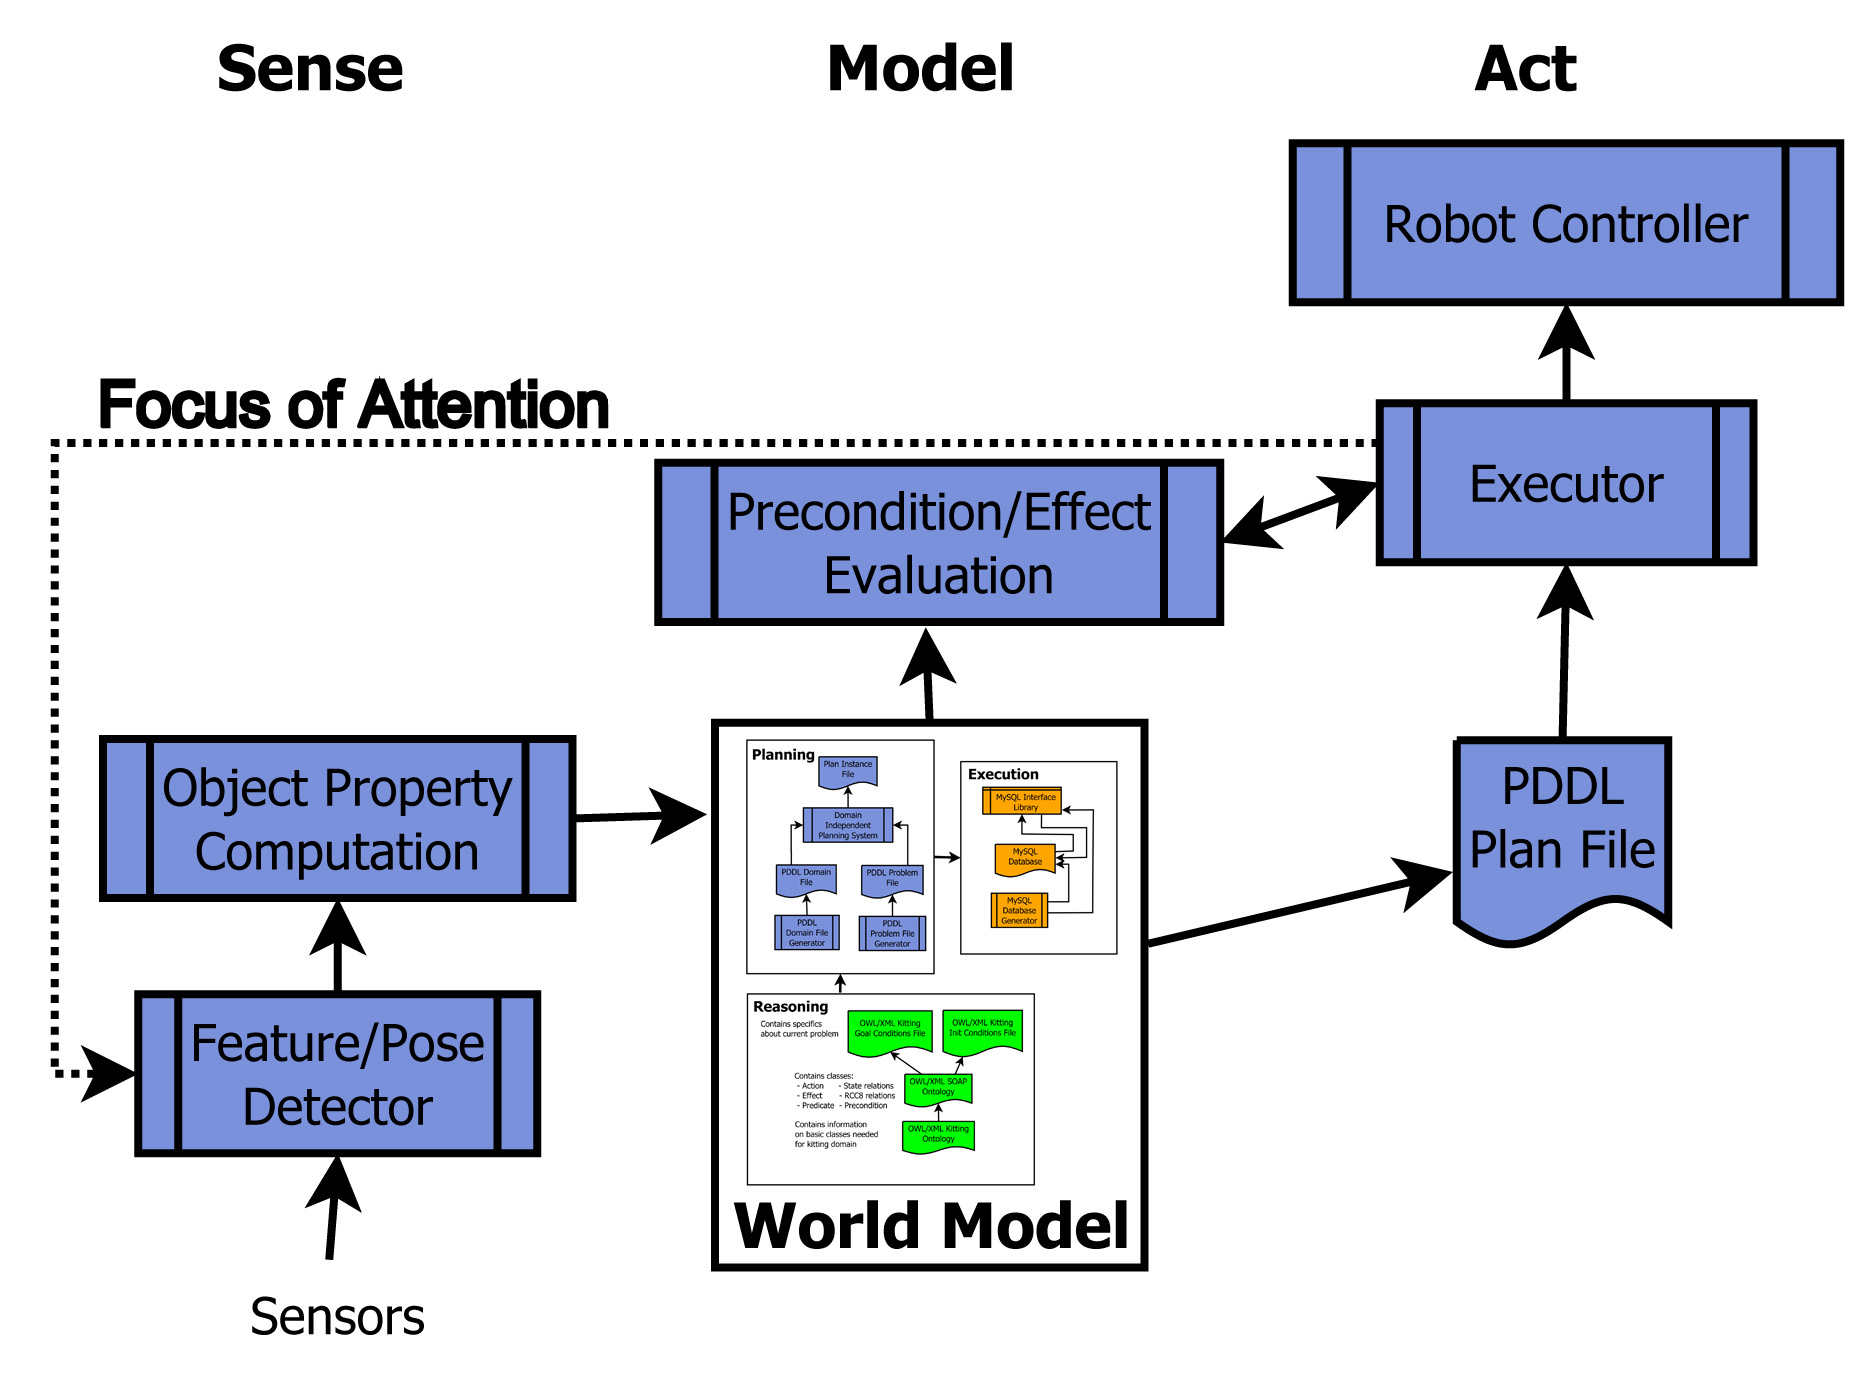
\includegraphics[width=8.5cm]{images/RITAExecution.jpg}
\caption{Major components that make up the Sense--Model--Act paradigm of the kitting station.}
\label{fig:SenseModelAct}
\end{center}
\end{figure}
\section{Paper Synopsis}
The special issue opens with two papers that examine various aspects of the IEEE Robotics 
and Automation Society's Robotics and Automation Working Group's ontology. The first paper
presents the Core Ontology for Robotics and Automation(CORA), while the second paper presents
details on the POS ontology that is designed for sharing spatial concepts in the Robotics 
and Automation domain.

These papers are followed by a set of articles that demonstrate human, robot cell collaboration
through the use of ontologies and software frameworks. The  intent of these papers is to 
provide mechanisms that allow users to better understand the process through their industrial
cell and to ease robot programming.

Three additional papers are presented that relate to robot programming and agility. These
papers present systems that attempt to enhance robot agility by allowing for dynamic
programming of the robot through the knowledge representation. Various protocols are
discussed along with metrics and test methods.  All of the papers in this section present
the sample domain of kit building to highlight their achievements.

From here, the special issue turns to use cases that utilize the knowledge representations for 
applications ranging from orthopedic surgery to intention recognition. Specific examples
of knowledge necessary for performing hip surgery, designing rehabilitation robots, and
using ontologies to determine the intentions of humans working together with robots
are examined.

\input{Acknowledgement}
%
%



%
% ---- Bibliography ----
%
%\bibliographystyle{plain}
%\bibliography{ontology}
\end{document}
